    \begin{figure*}[t!]
        %%%%%%%%%%% Example 1 %%%%%%%%%%%%%%%
        \begin{minipage}{1.0\linewidth}
        \end{minipage}
        % QUERY image
        \begin{minipage}{0.34\linewidth}
            \centering
            \vspace{5mm}
            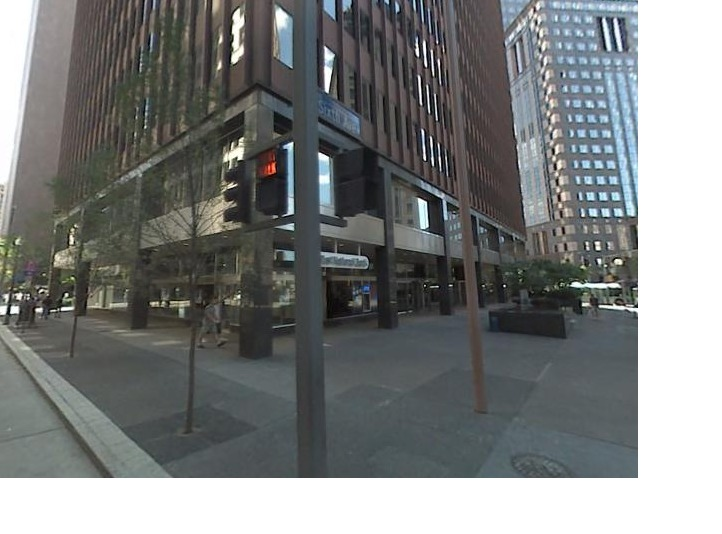
\includegraphics[height=40mm]{imgs/ex1/query.jpg}
        \end{minipage}
        % Retrieved images
        \begin{minipage}{0.75\linewidth}
            % FV e-SVM
            \begin{minipage}{\linewidth} 
                \colorbox{myGreen}{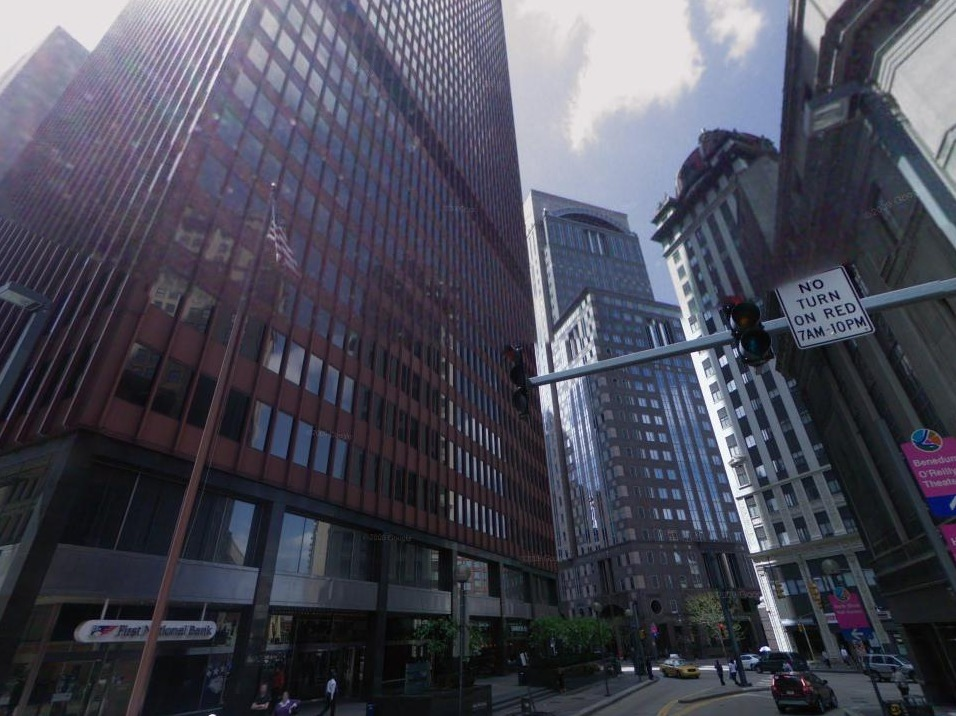
\includegraphics[height=16mm]{imgs/ex1/FVsvm1.jpg}}
                \colorbox{myGreen}{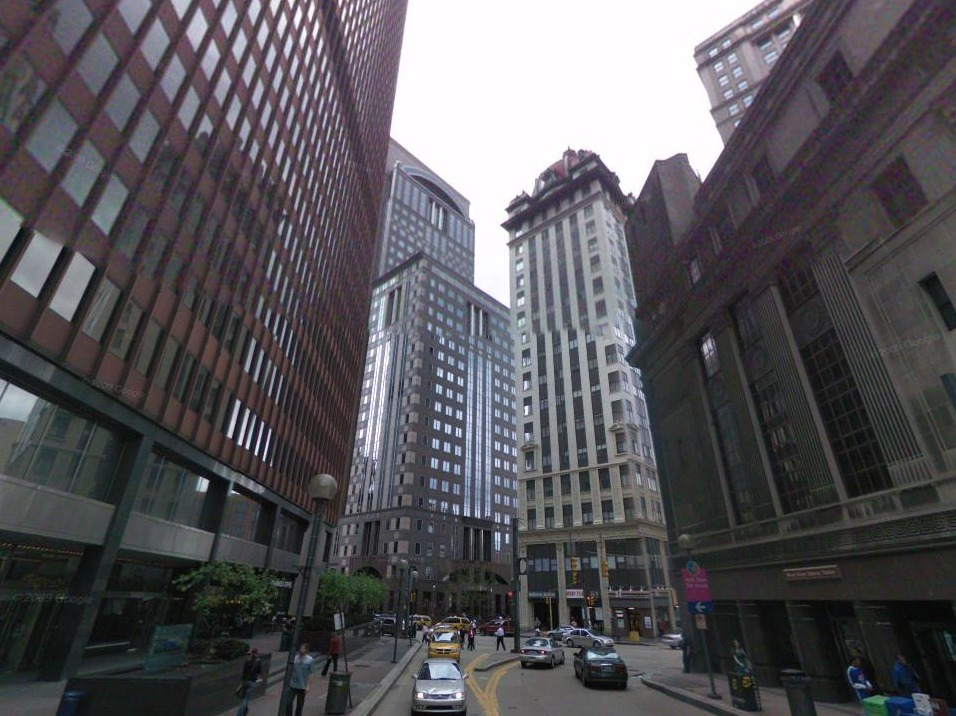
\includegraphics[height=16mm]{imgs/ex1/FVsvm2.jpg}}
                \colorbox{myGreen}{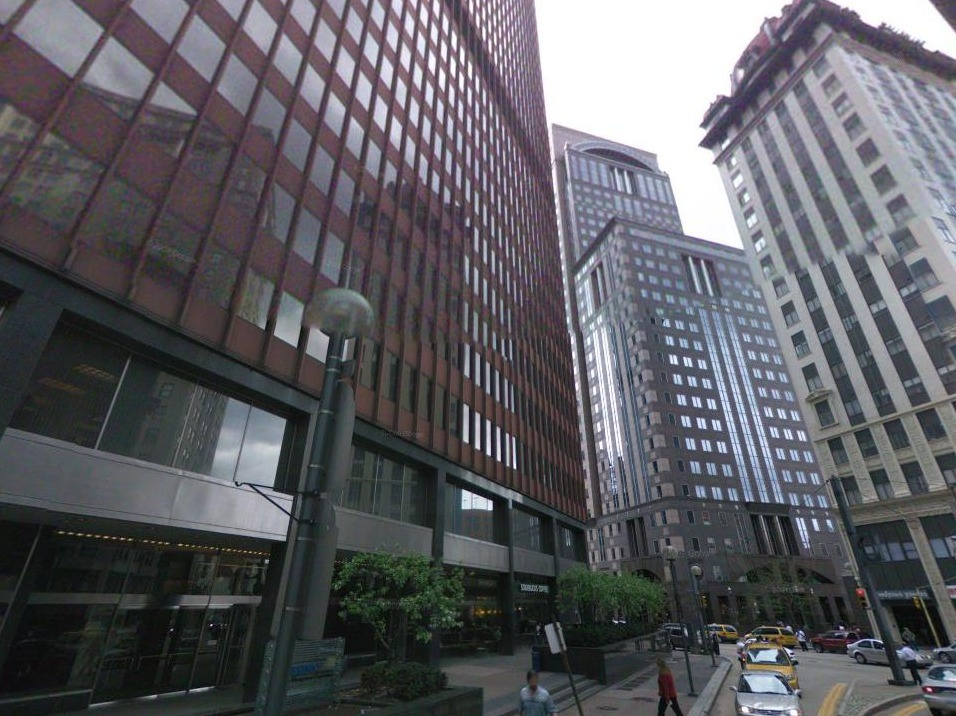
\includegraphics[height=16mm]{imgs/ex1/FVsvm3.jpg}}
                \colorbox{myGreen}{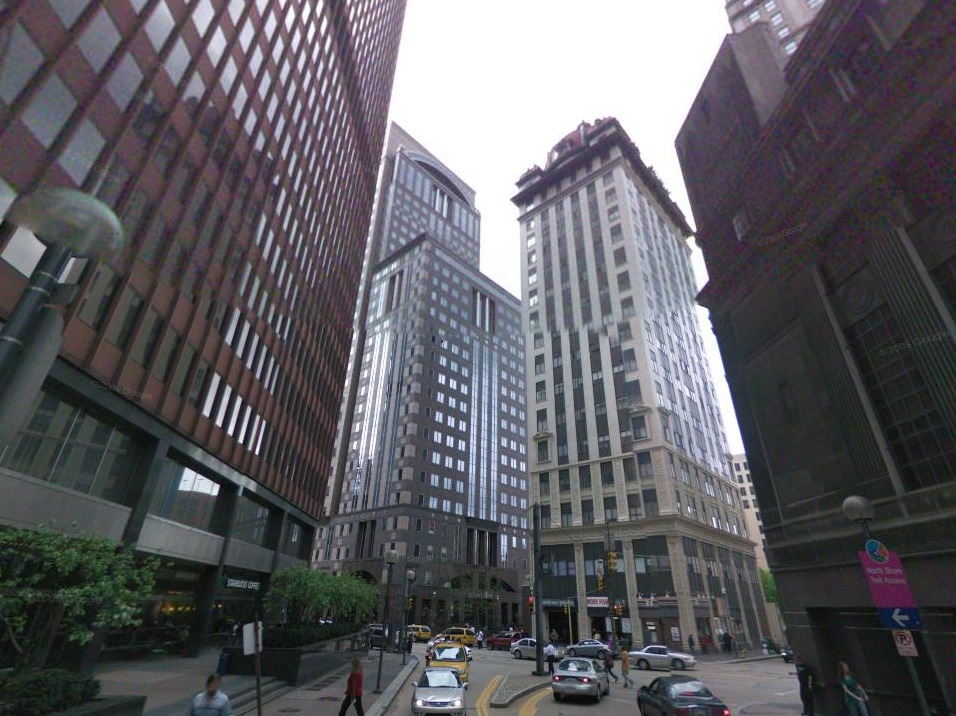
\includegraphics[height=16mm]{imgs/ex1/FVsvm4.jpg}}
            \end{minipage}
            \\
            \begin{minipage}{\linewidth}
                \colorbox{myRed}{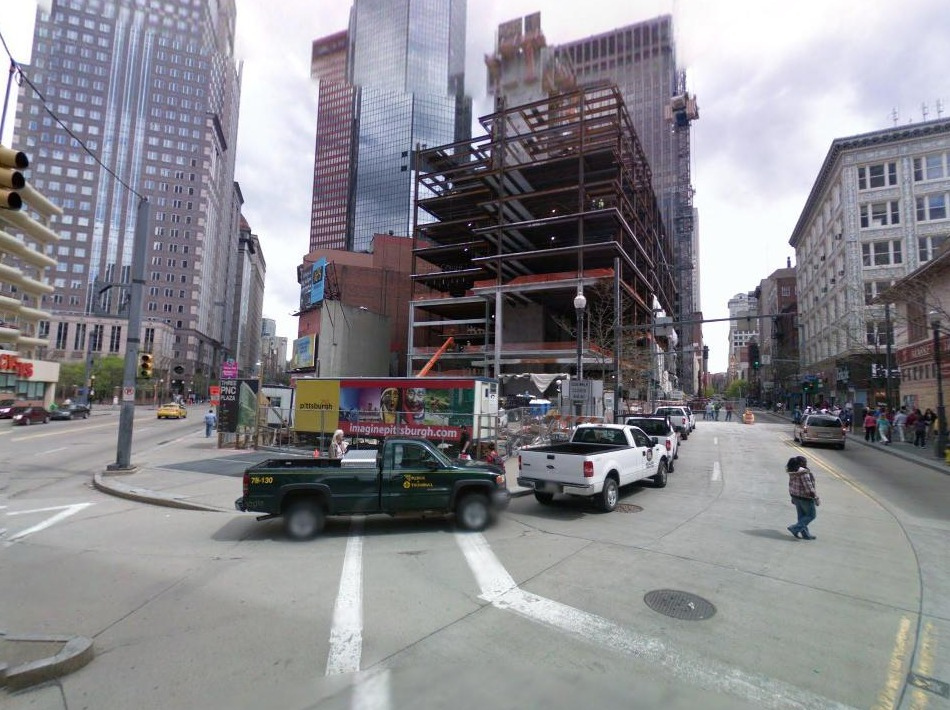
\includegraphics[height=16mm]{imgs/ex1/FV1.jpg}}
                \colorbox{myRed}{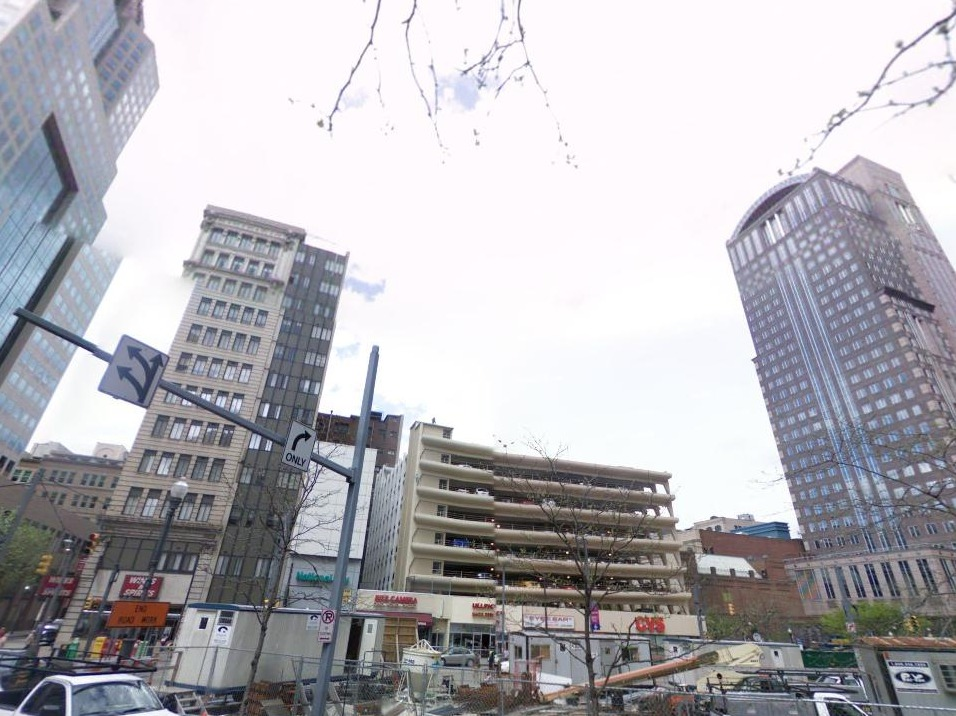
\includegraphics[height=16mm]{imgs/ex1/FV2.jpg}}
                \colorbox{myRed}{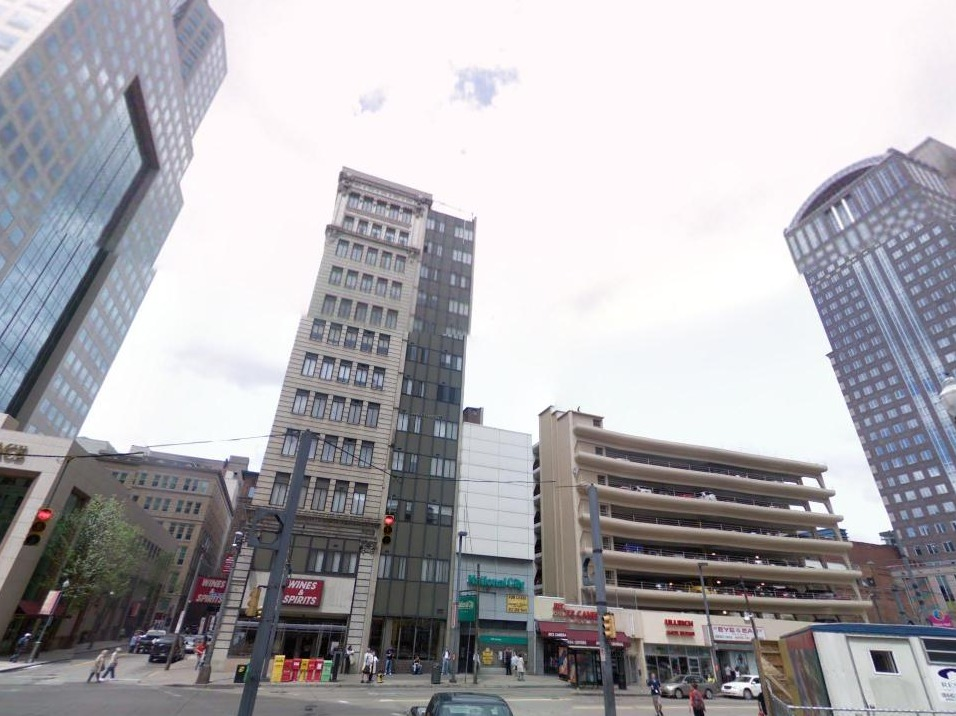
\includegraphics[height=16mm]{imgs/ex1/FV3.jpg}}
                \colorbox{myRed}{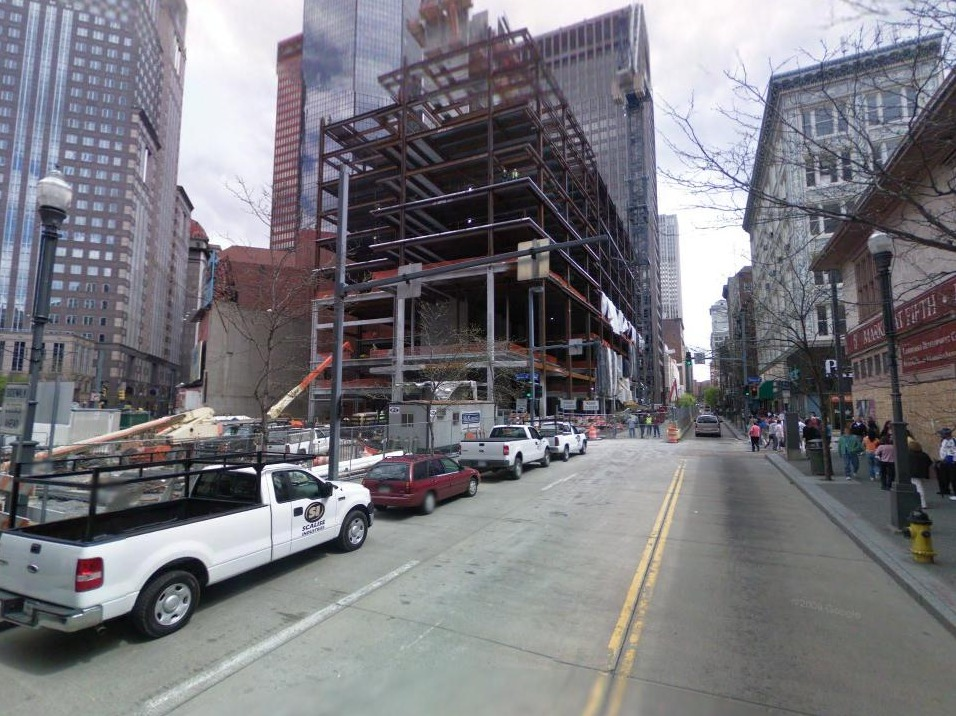
\includegraphics[height=16mm]{imgs/ex1/FV4.jpg}}
            \end{minipage} 
        \end{minipage}
        \\
        %%%%%%%%%%% Example 2 %%%%%%%%%%%%%%%
        \begin{minipage}{0.34\linewidth}
            \centering
            \vspace{0mm}
            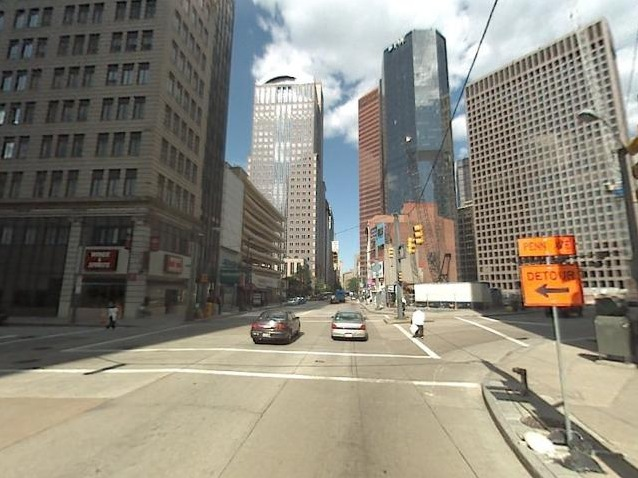
\includegraphics[height=36mm]{imgs/ex2/query.jpg}
        \end{minipage}
        % Retrieved images
        \begin{minipage}{0.75\linewidth}
            % FV e-SVM
            \begin{minipage}{\linewidth} 
                \colorbox{myGreen}{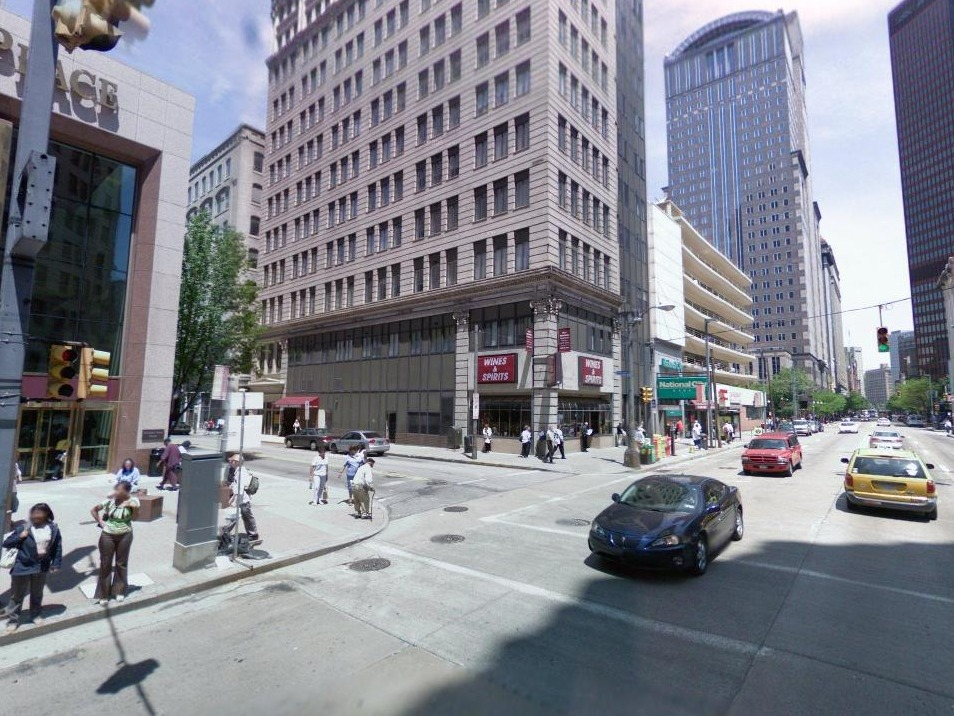
\includegraphics[height=16mm]{imgs/ex2/FVsvm1.jpg}}
                \colorbox{myGreen}{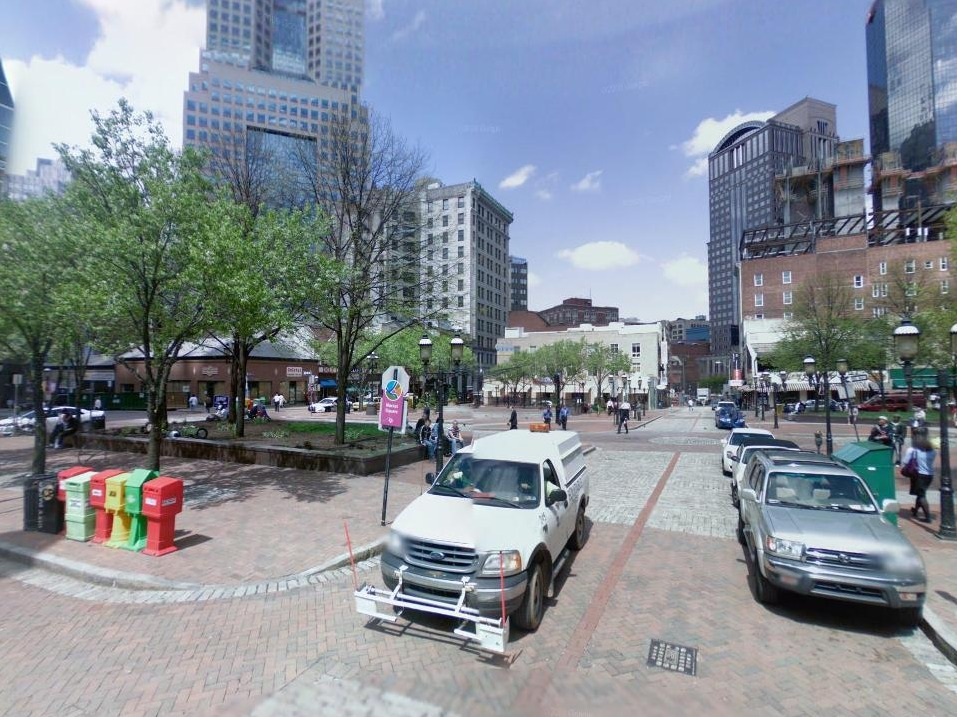
\includegraphics[height=16mm]{imgs/ex2/FVsvm2.jpg}}
                \colorbox{myGreen}{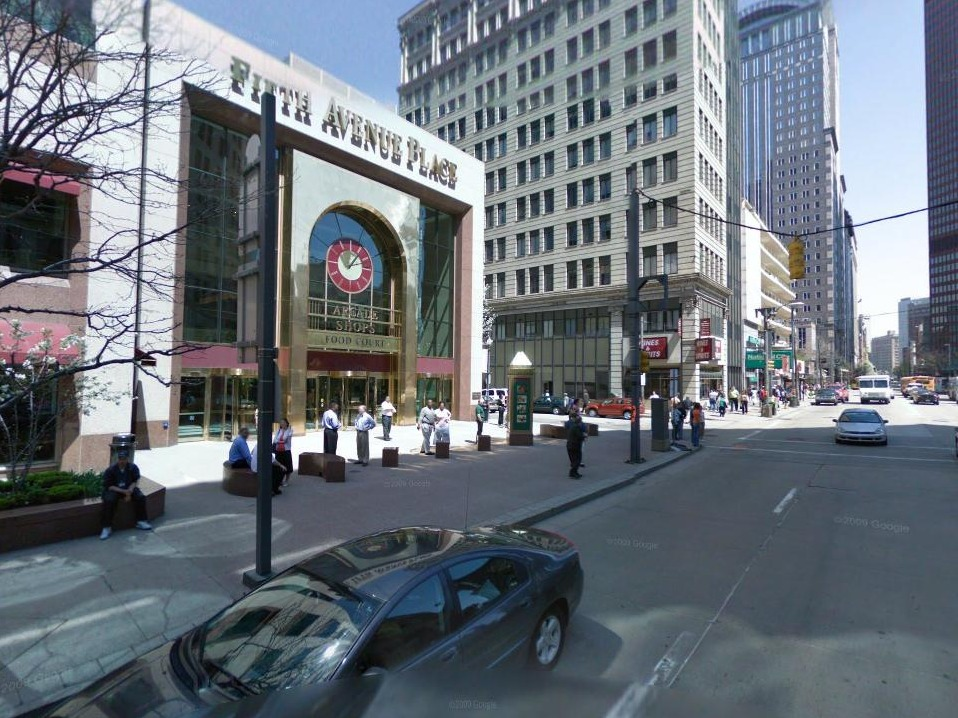
\includegraphics[height=16mm]{imgs/ex2/FVsvm3.jpg}}
                \colorbox{myGreen}{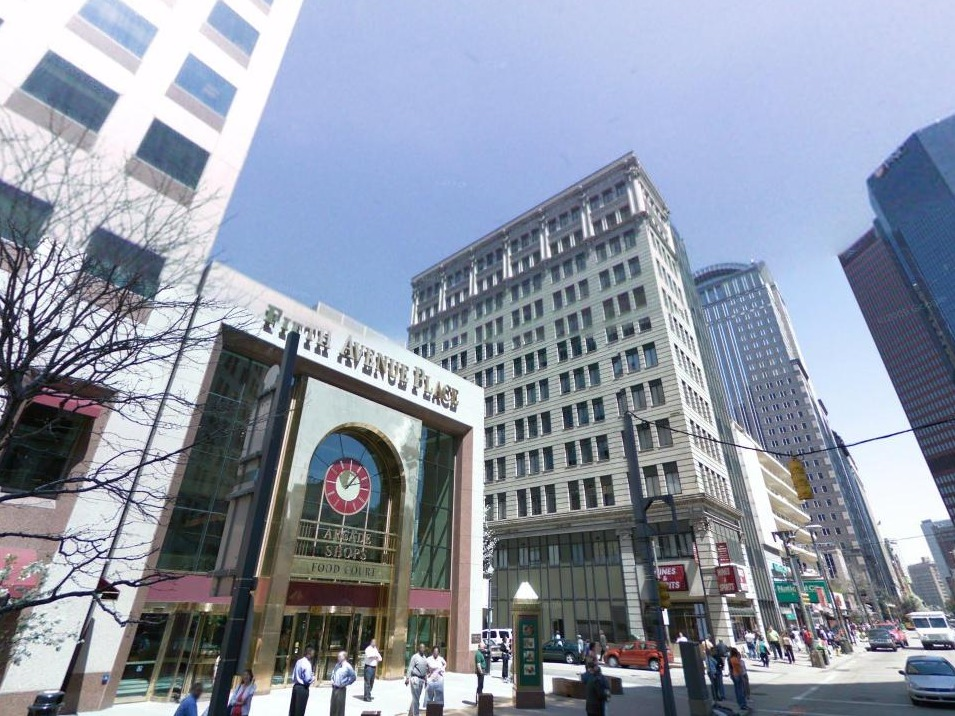
\includegraphics[height=16mm]{imgs/ex2/FVsvm4.jpg}}
            \end{minipage}
            \\
            \begin{minipage}{\linewidth}
                \colorbox{myRed}{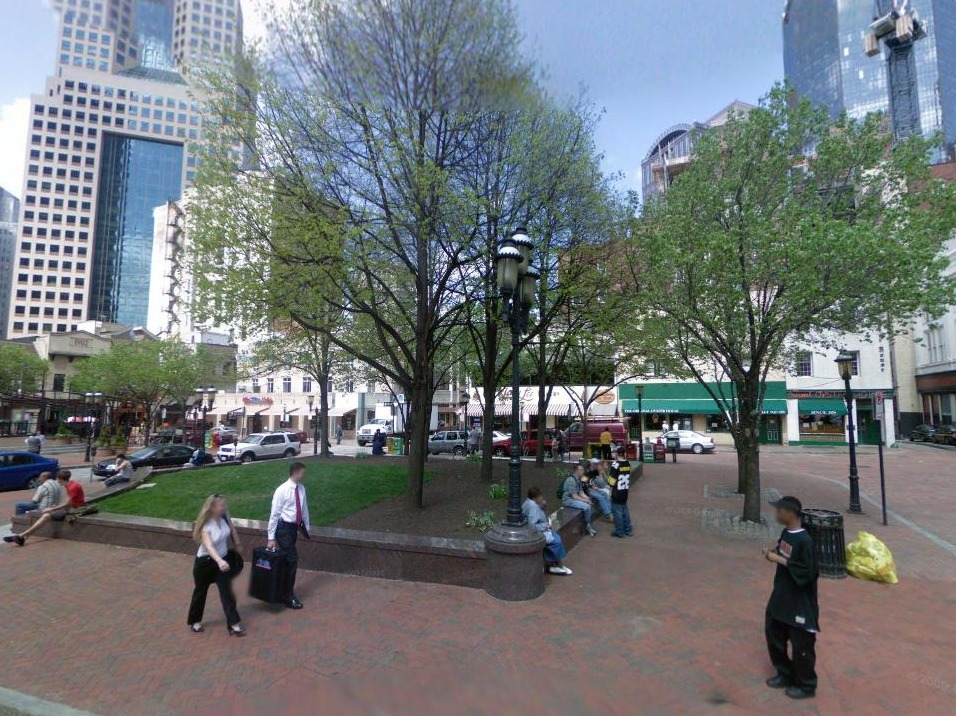
\includegraphics[height=16mm]{imgs/ex2/FV1.jpg}}
                \colorbox{myRed}{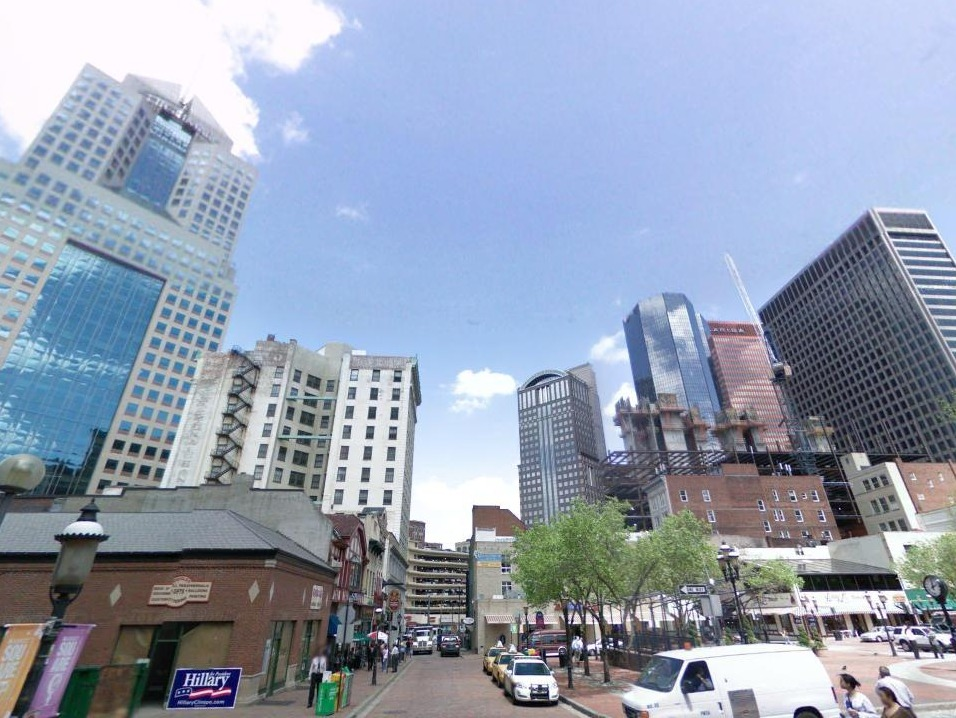
\includegraphics[height=16mm]{imgs/ex2/FV2.jpg}}
                \colorbox{myRed}{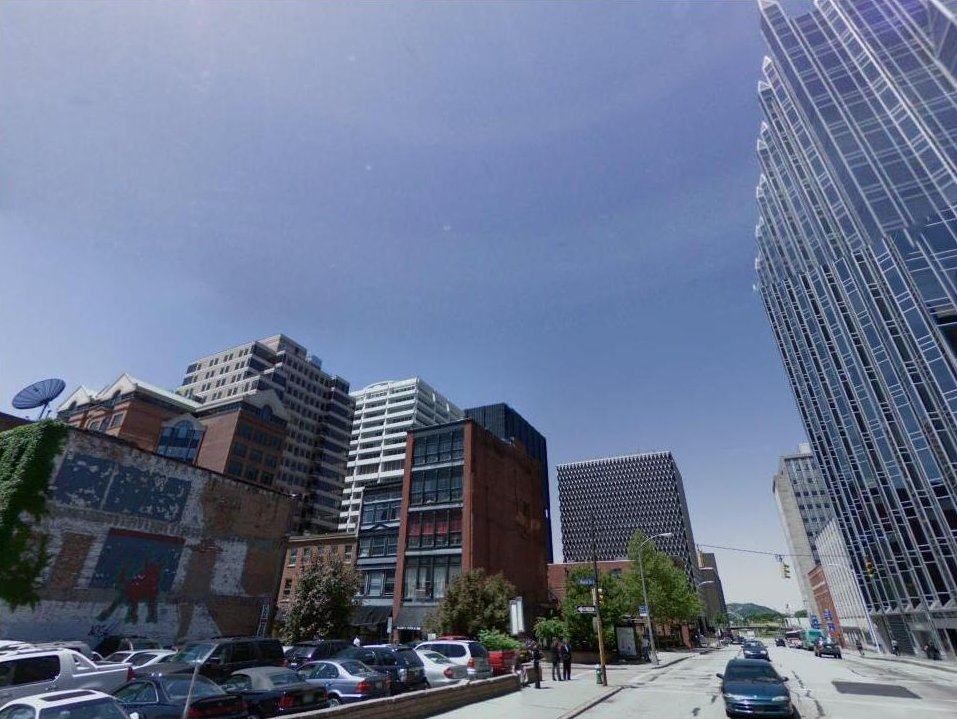
\includegraphics[height=16mm]{imgs/ex2/FV3.jpg}}
                \colorbox{myRed}{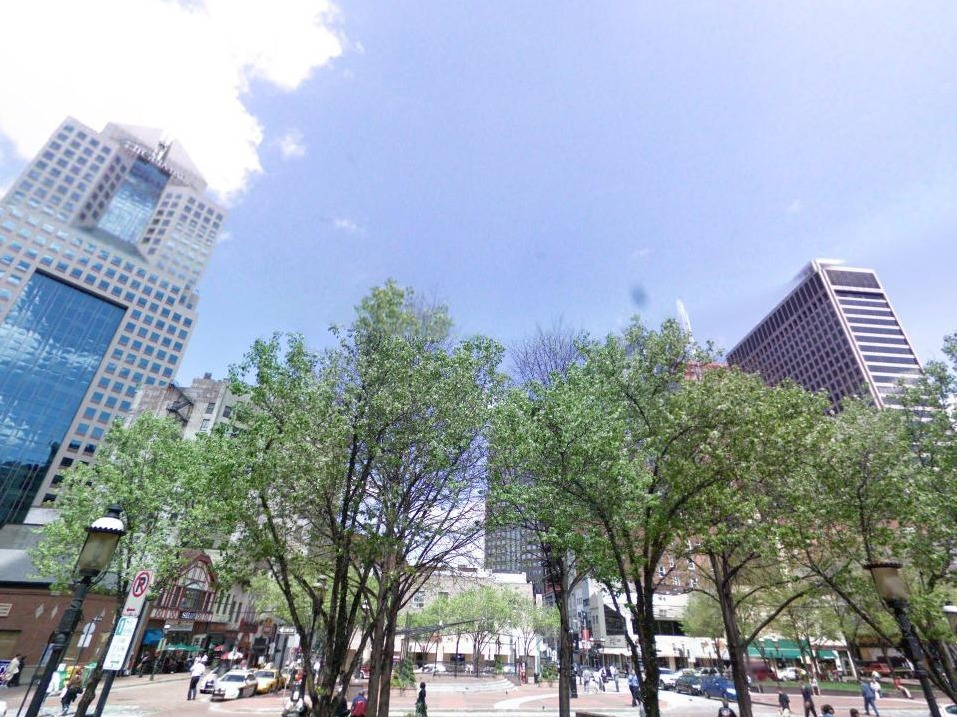
\includegraphics[height=16mm]{imgs/ex2/FV4.jpg}}
            \end{minipage} 
        \end{minipage}
        \vspace{3mm}
        \\
        %%%%%%%%%%% Example 3 %%%%%%%%%%%%%%%
        \begin{minipage}{0.34\linewidth}
            \centering
            \vspace{0mm}
            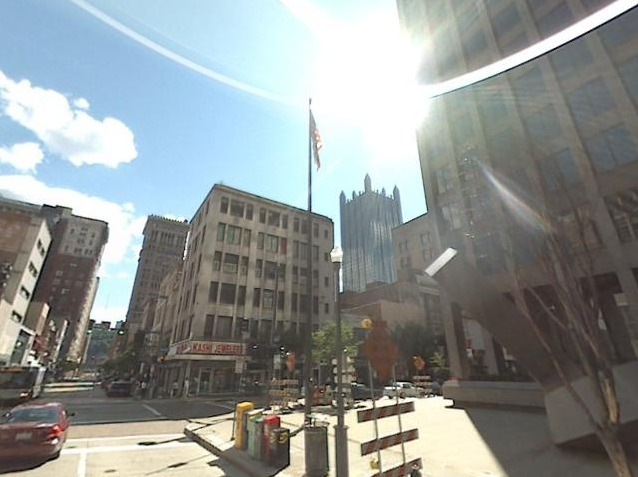
\includegraphics[height=36mm]{imgs/ex3/query.jpg}
        \end{minipage}
        % Retrieved images
        \begin{minipage}{0.75\linewidth}
            % FV e-SVM
            \begin{minipage}{\linewidth} 
                \colorbox{myGreen}{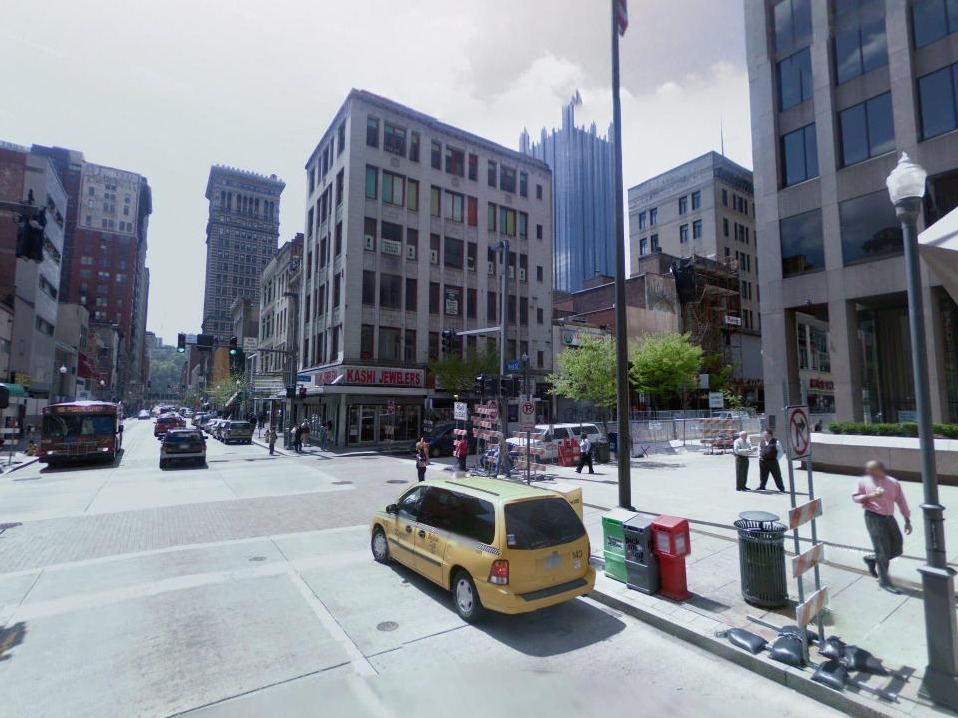
\includegraphics[height=16mm]{imgs/ex3/FVsvm1.jpg}}
                \colorbox{myRed}{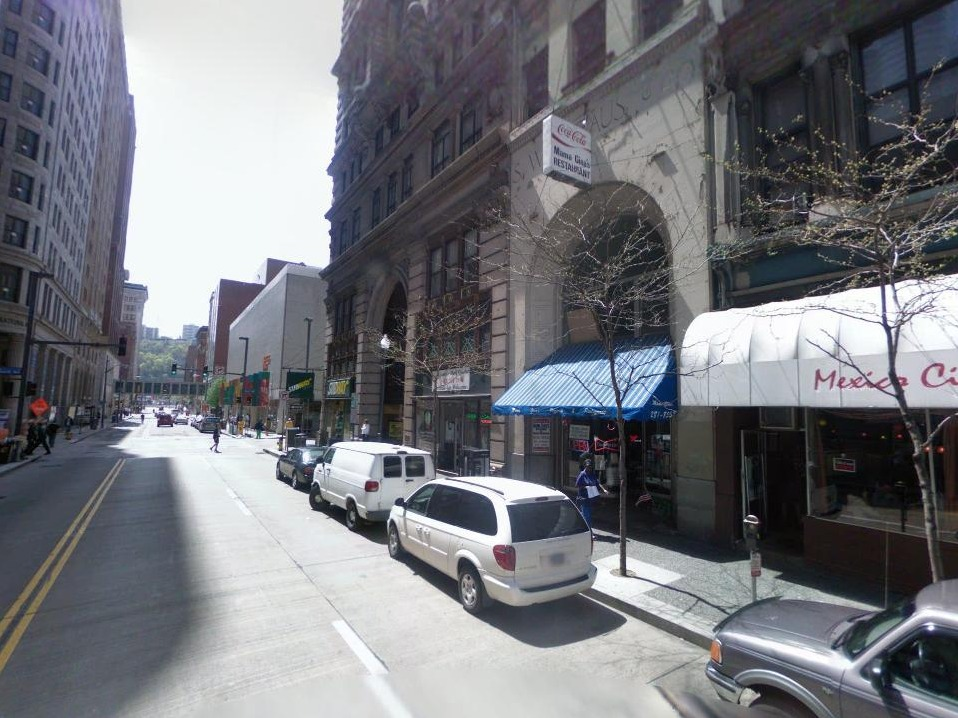
\includegraphics[height=16mm]{imgs/ex3/FVsvm2.jpg}}
                \colorbox{myGreen}{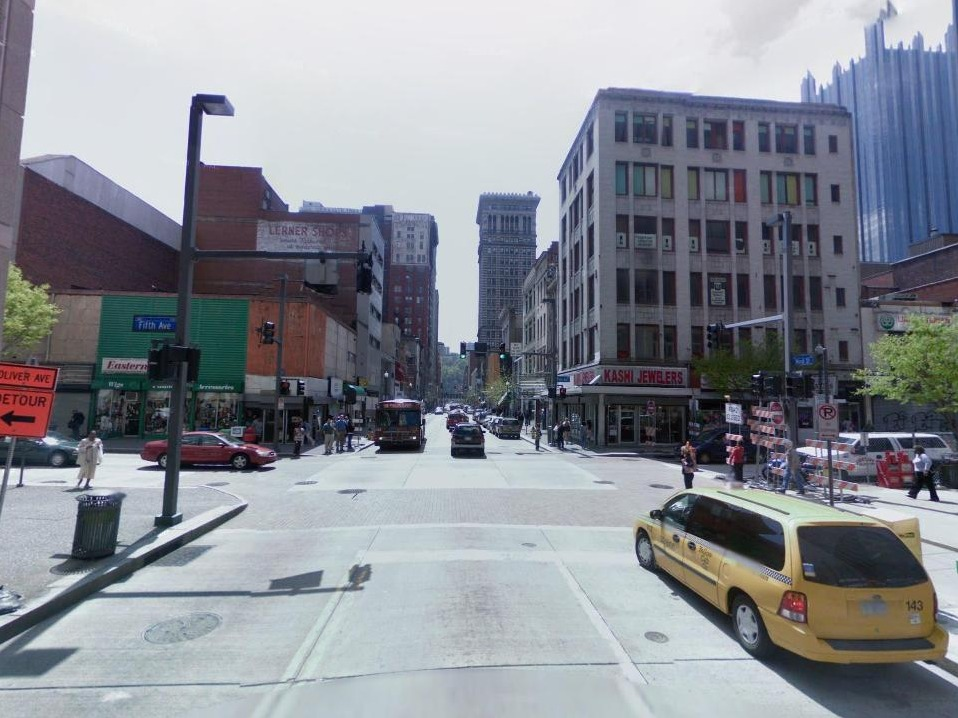
\includegraphics[height=16mm]{imgs/ex3/FVsvm5.jpg}}
                \colorbox{myGreen}{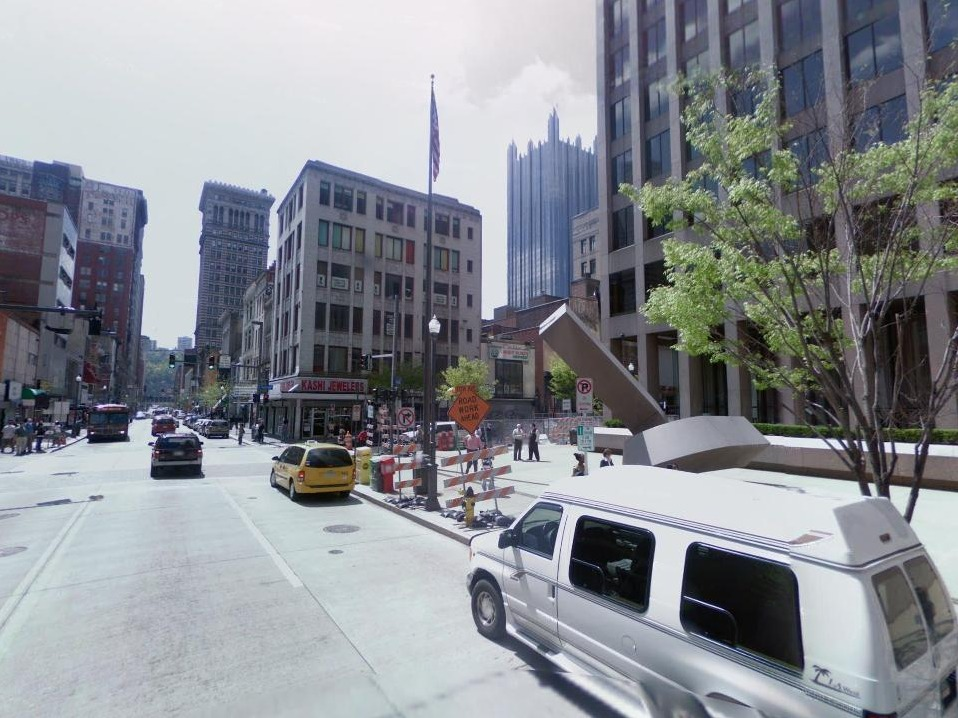
\includegraphics[height=16mm]{imgs/ex3/FVsvm4.jpg}}
            \end{minipage}
            \\
            \begin{minipage}{\linewidth}
                \colorbox{myRed}{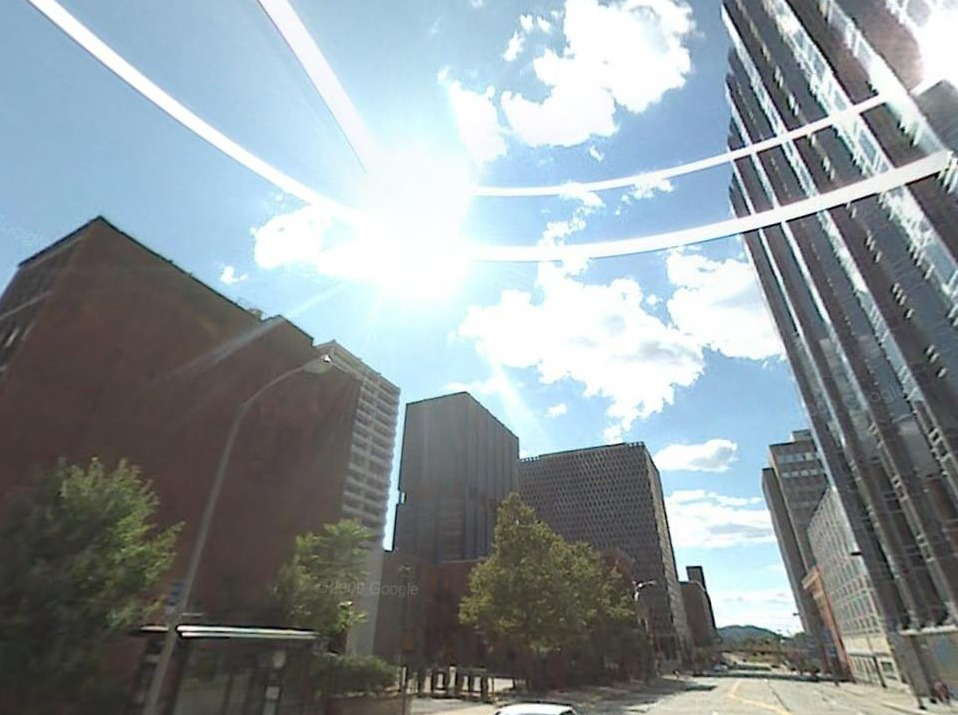
\includegraphics[height=16mm]{imgs/ex3/FV1.jpg}}
                \colorbox{myGreen}{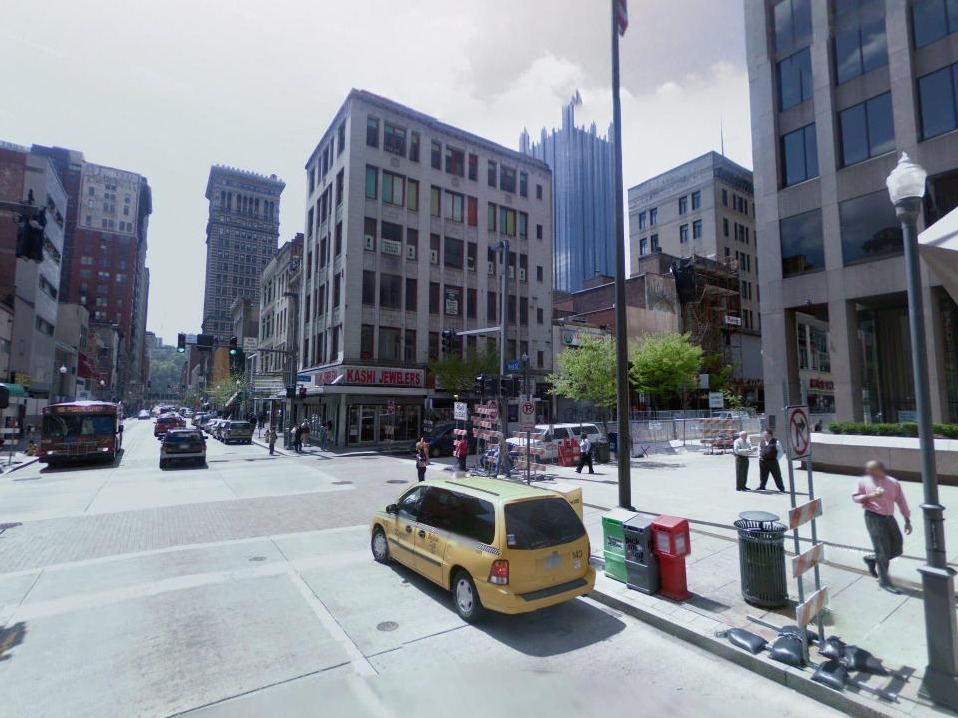
\includegraphics[height=16mm]{imgs/ex3/FV2.jpg}}
                \colorbox{myRed}{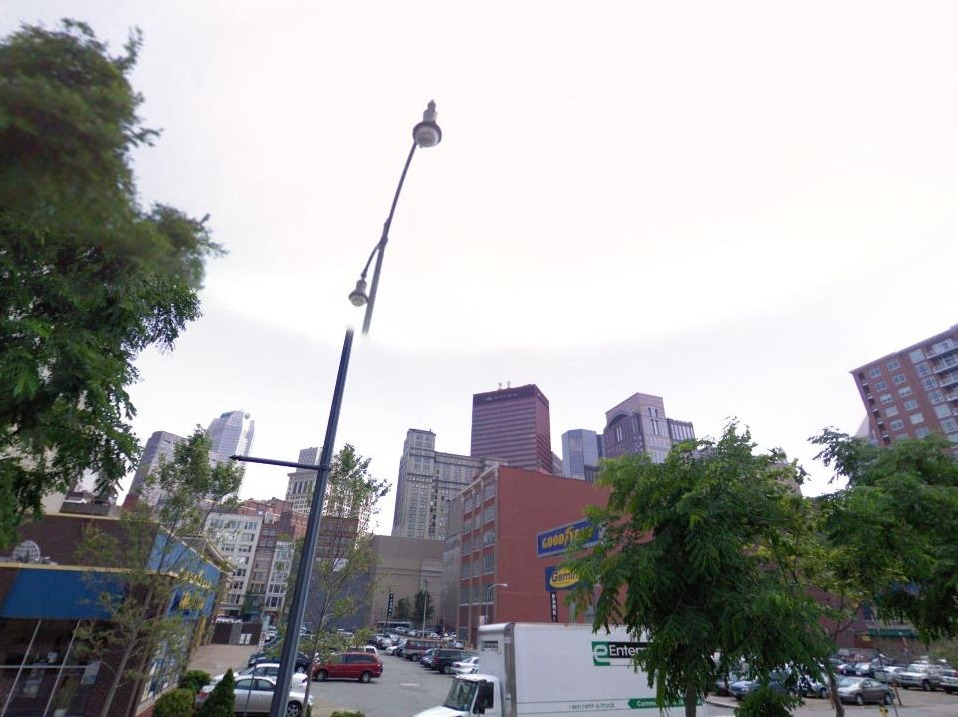
\includegraphics[height=16mm]{imgs/ex3/FV3.jpg}}
                \colorbox{myRed}{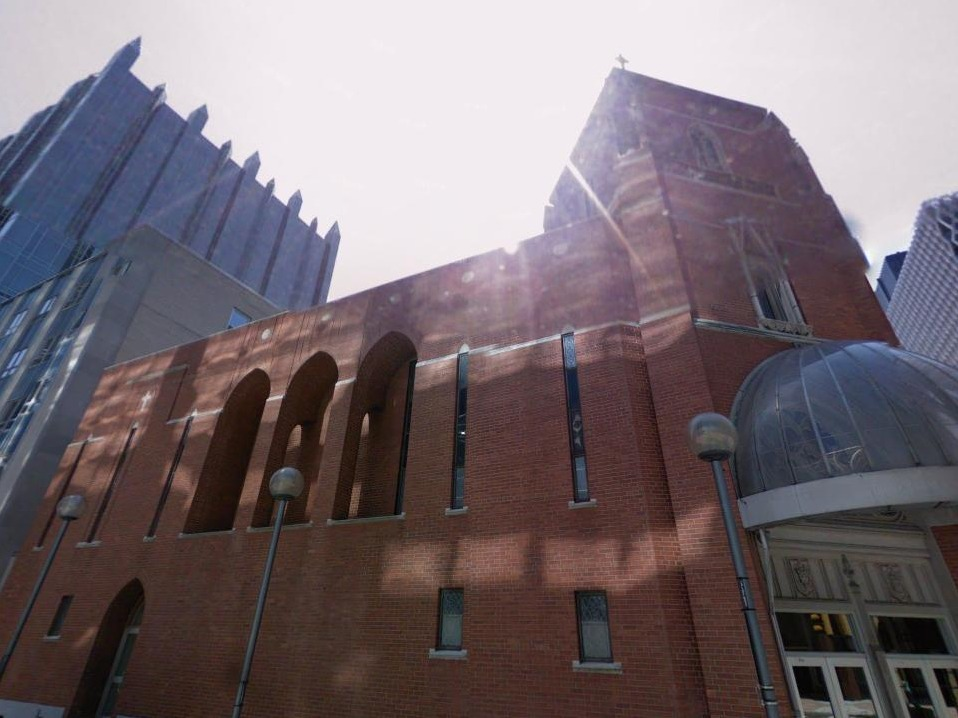
\includegraphics[height=16mm]{imgs/ex3/FV4.jpg}}
            \end{minipage} 
        \end{minipage}
        \vspace{3mm}
        \\
        %%%%%%%%%%% Example 4 %%%%%%%%%%%%%%%
        \begin{minipage}{0.34\linewidth}
            \centering
            \vspace{0mm}
            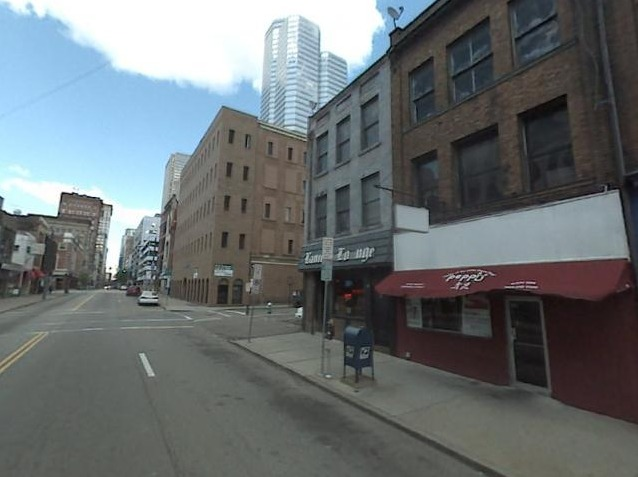
\includegraphics[height=36mm]{imgs/ex4/query.jpg}
        \end{minipage}
        % Retrieved images
        \begin{minipage}{0.75\linewidth}
            % FV e-SVM
            \begin{minipage}{\linewidth} 
                \colorbox{myGreen}{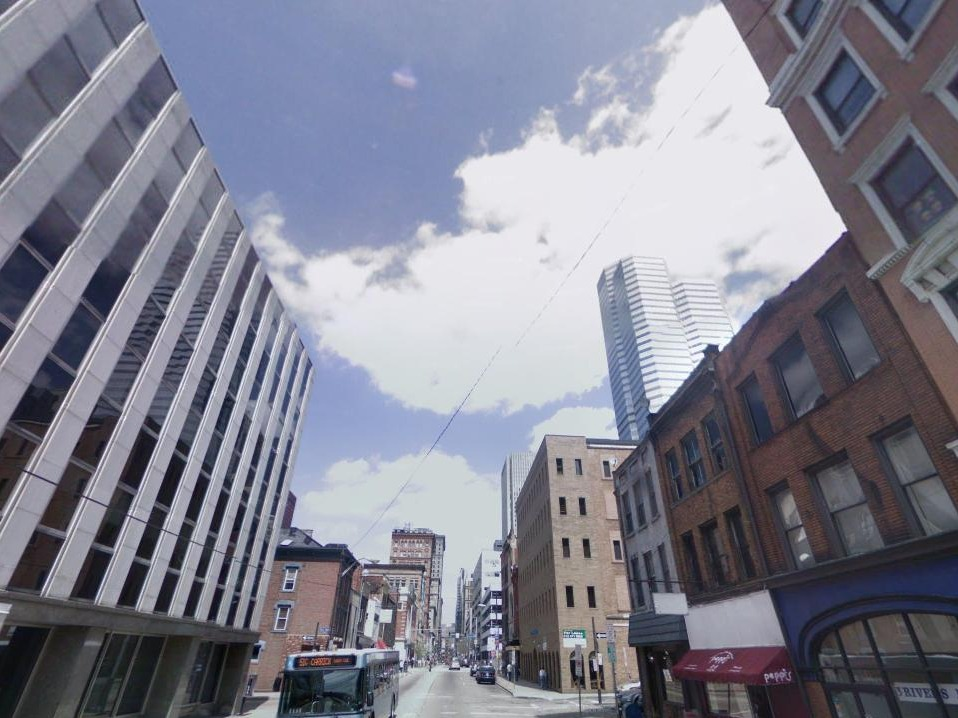
\includegraphics[height=16mm]{imgs/ex4/FVsvm1.jpg}}
                \colorbox{myRed}{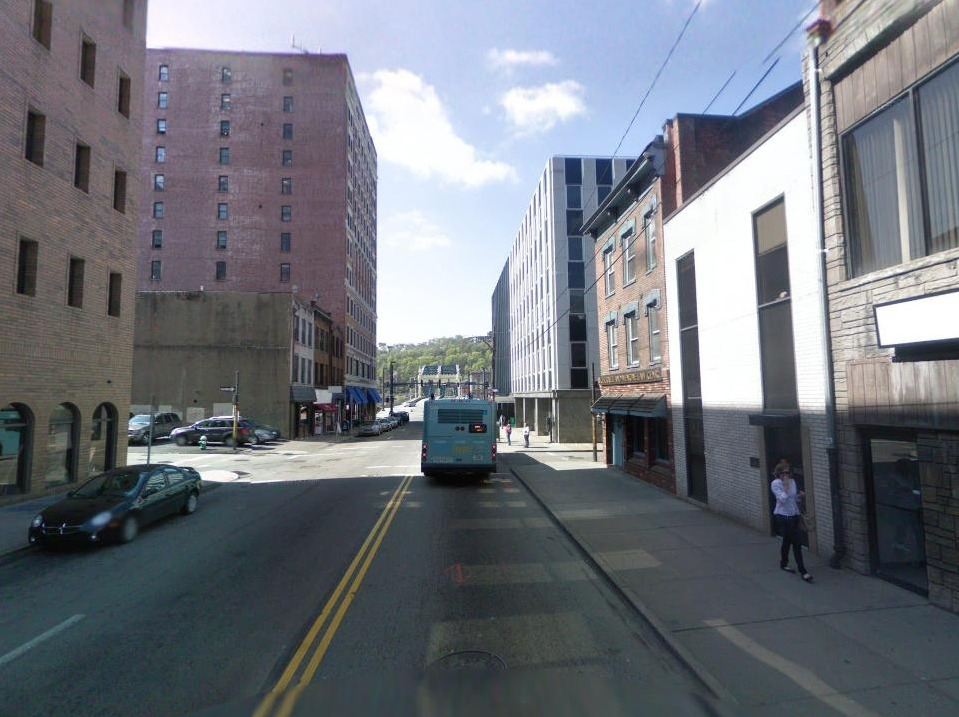
\includegraphics[height=16mm]{imgs/ex4/FVsvm2.jpg}}
                \colorbox{myGreen}{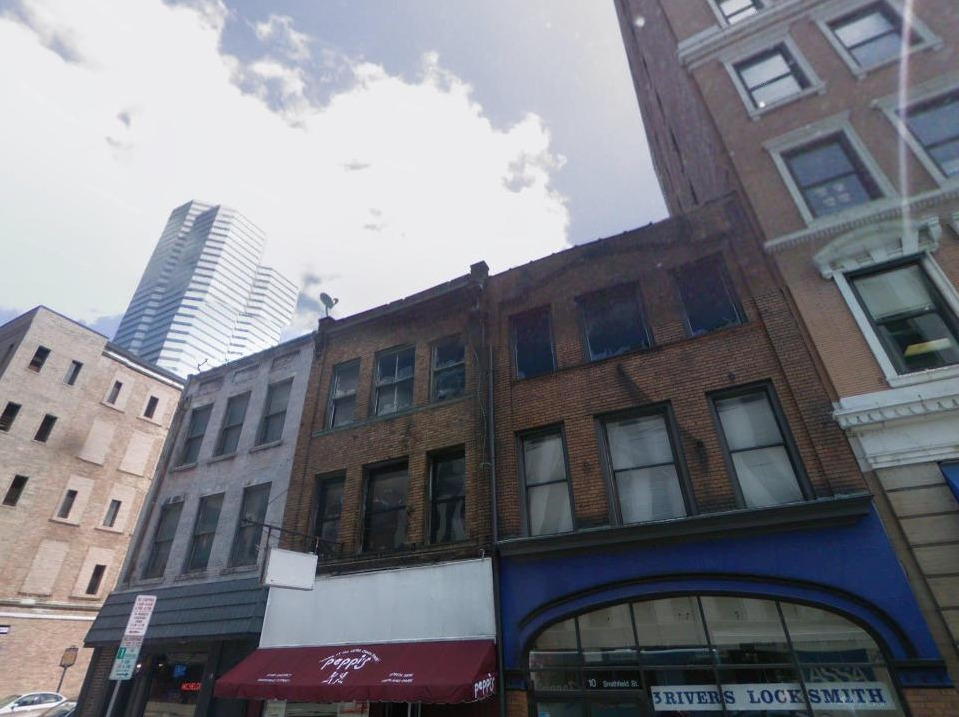
\includegraphics[height=16mm]{imgs/ex4/FVsvm5.jpg}}
                \colorbox{myGreen}{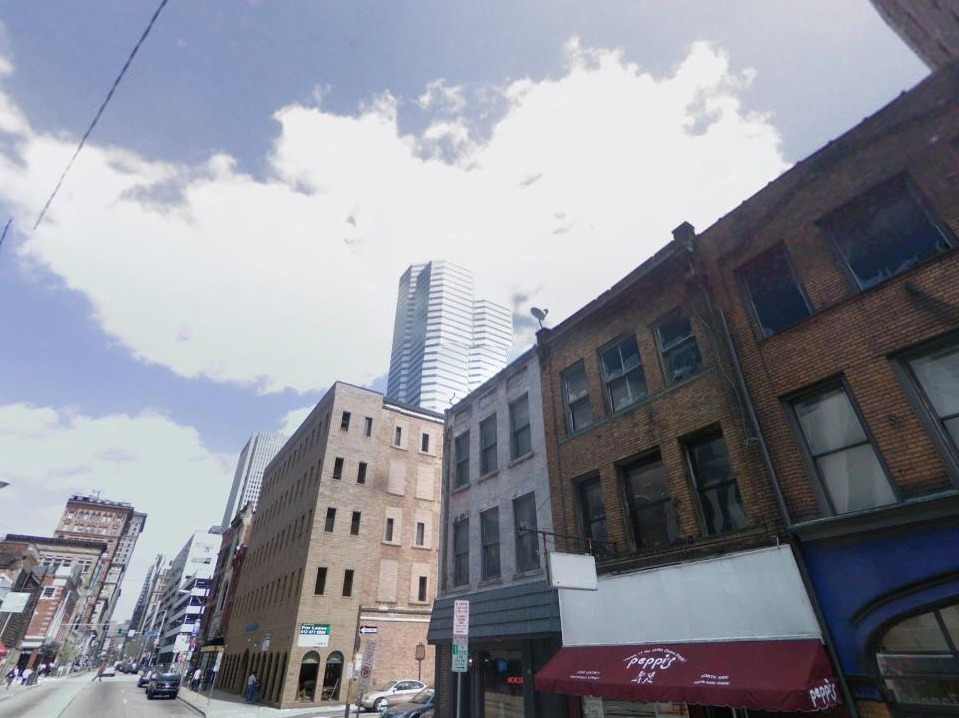
\includegraphics[height=16mm]{imgs/ex4/FVsvm4.jpg}}
            \end{minipage}
            \\
            \begin{minipage}{\linewidth}
                \colorbox{myRed}{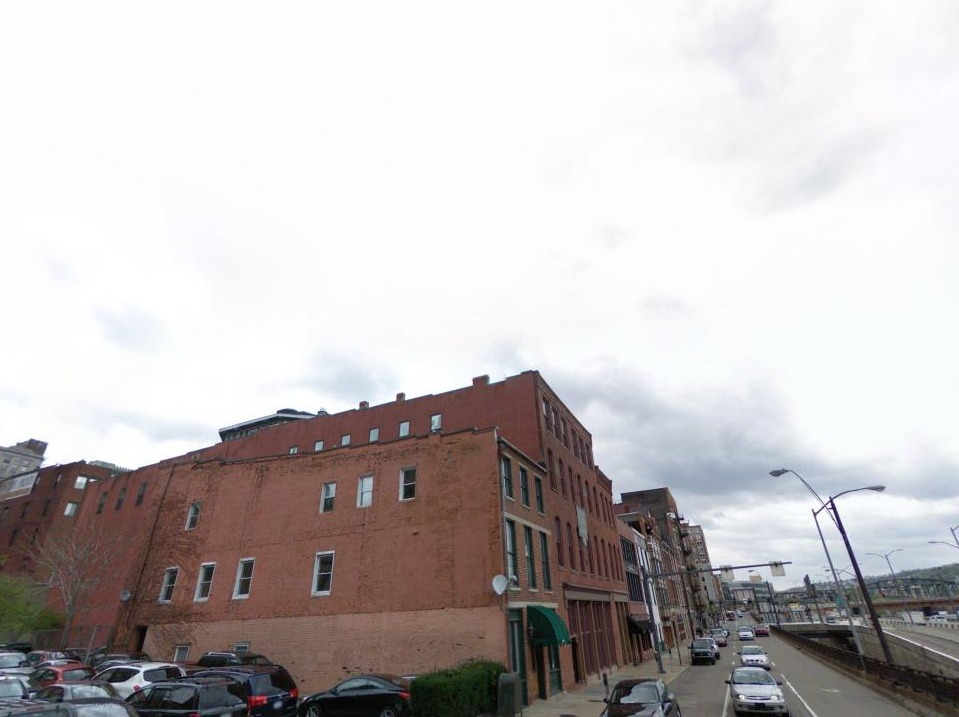
\includegraphics[height=16mm]{imgs/ex4/FV1.jpg}}
                \colorbox{myGreen}{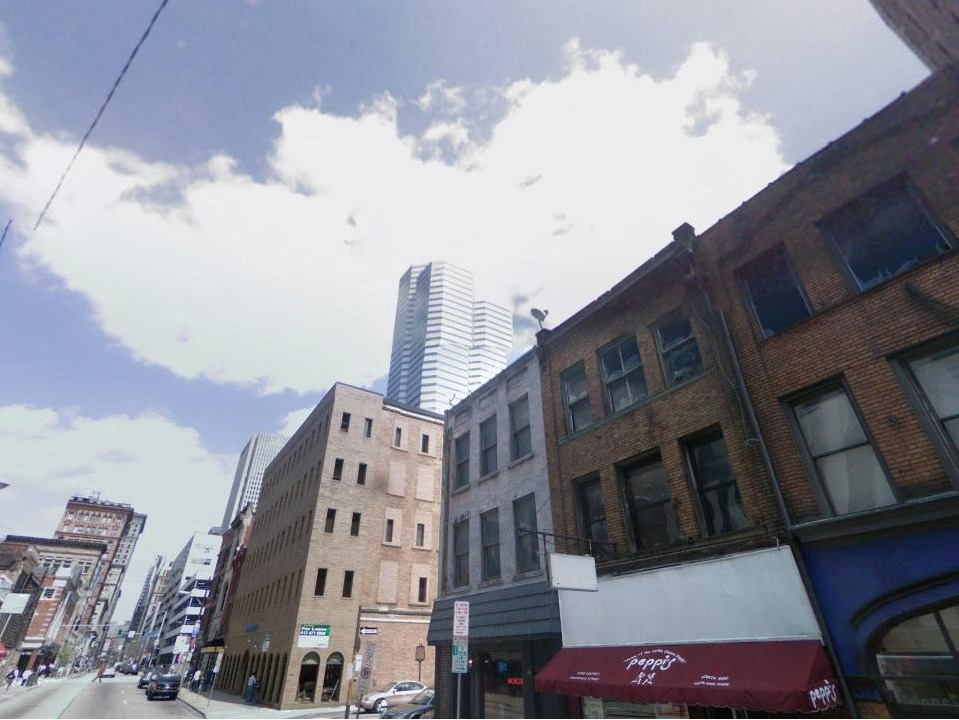
\includegraphics[height=16mm]{imgs/ex4/FV2.jpg}}
                \colorbox{myRed}{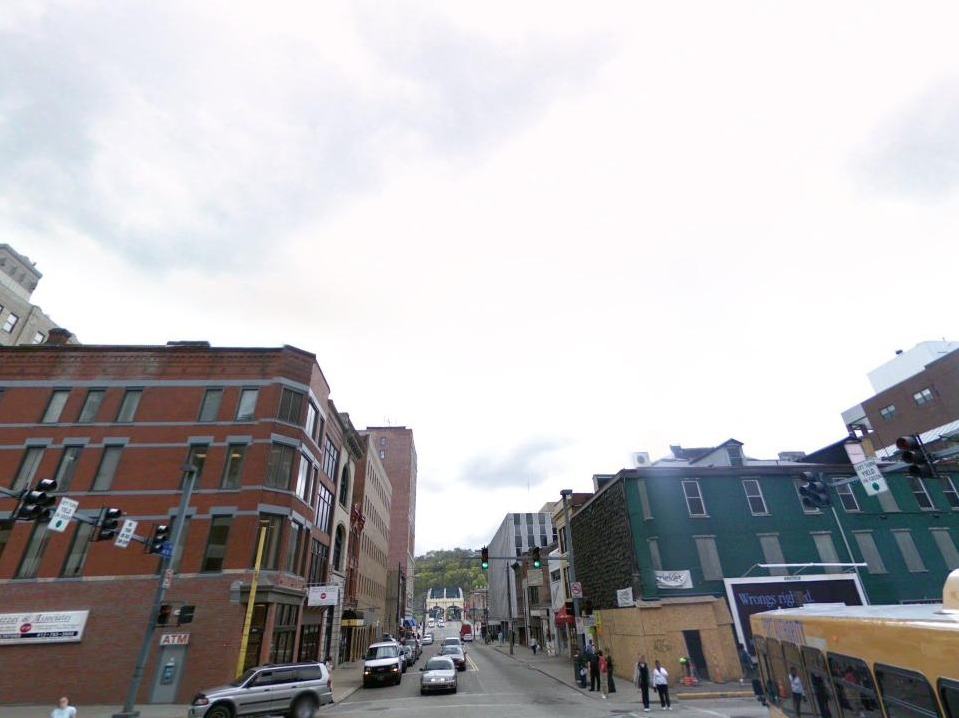
\includegraphics[height=16mm]{imgs/ex4/FV3.jpg}}
                \colorbox{myRed}{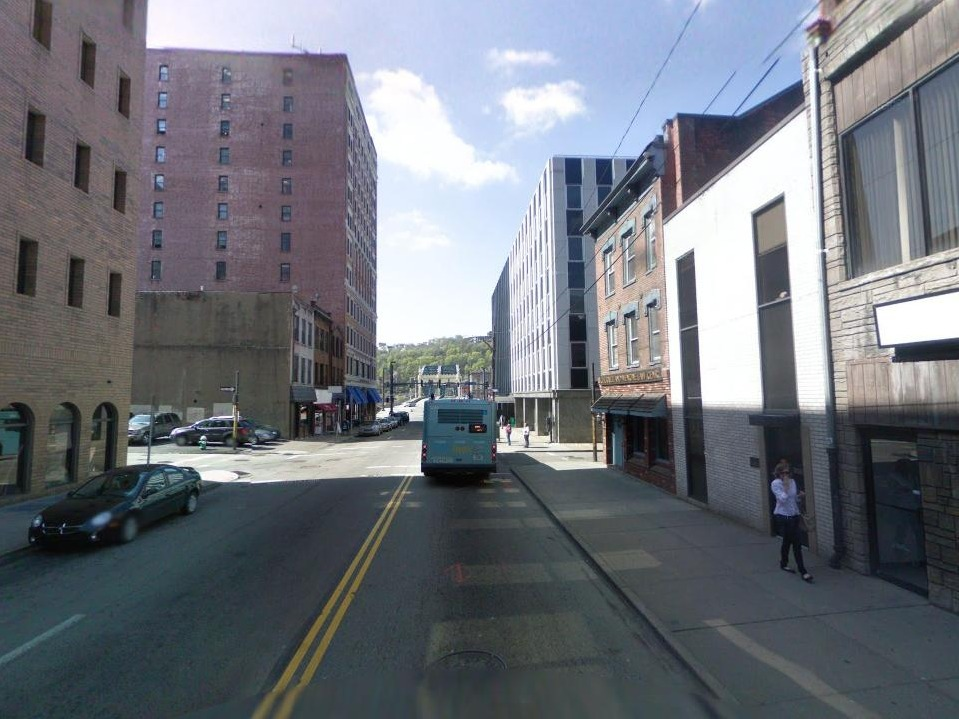
\includegraphics[height=16mm]{imgs/ex4/FV4.jpg}}
            \end{minipage} 
        \end{minipage}
        %%%%%%%%%%%%%%%%%%%%%%%%%%%%%%%%%%%%%
        \caption{
            Each example shows a query image (left) together with correct (green) and incorrect (red) matches from the database obtained by \emph{w-norm} method (top) and the raw Fisher vector descriptor baseline (bottom). For each method we show the top 4 matches from the database using 128-dimensional descriptors.        
        }
        \label{fig:images}
    \end{figure*}